\section*{1. Graf for funktion}
\textbf{Opgavebeskrivelse:}
\begin{color}{AAUblue2}
%
Tegn grafen for funktionen $f(x)$ fra (1) for forskellige valg af parametrene $h_0$ og $\lambda$.
Forsøg at forklare hvilken effekt parametrene har på kurvens form.
% 
\end{color}
\\\\
%
Kode implementeringen finde i appendix \ref{app:1.1}.
% 
Ændringer i $h_0$ viser sig kun at ændre på højden af kædelinjen, men påvirker ikke selve kædens form. 
%
\begin{figure}[h!]
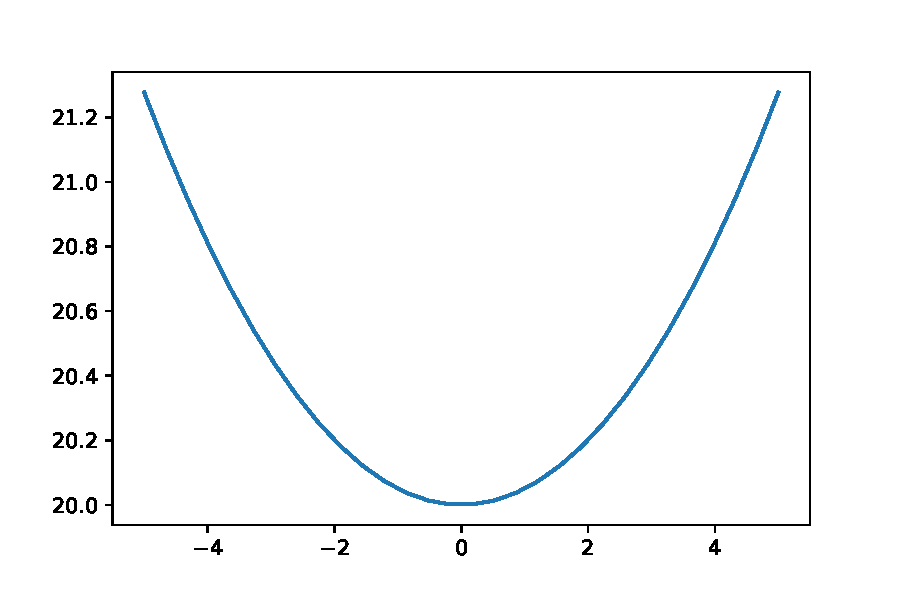
\includegraphics[scale=0.5]{code/fig1}
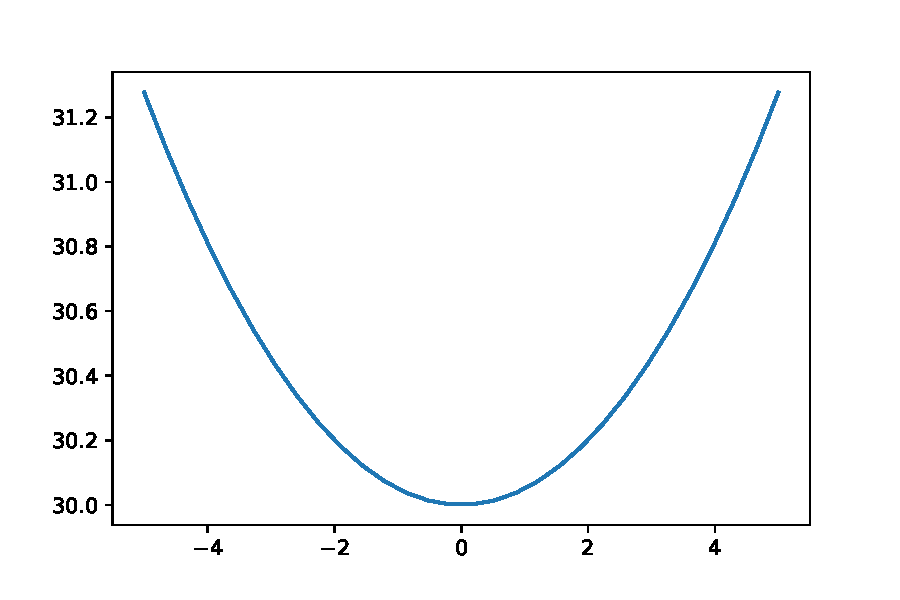
\includegraphics[scale=0.5]{code/fig2}
\caption{Det ses at en ændring fra $h_0=10$ til $h_0=20$ kun ændrer højden af kæden men ikke formen.}
\end{figure}
%
\begin{figure}[h!]
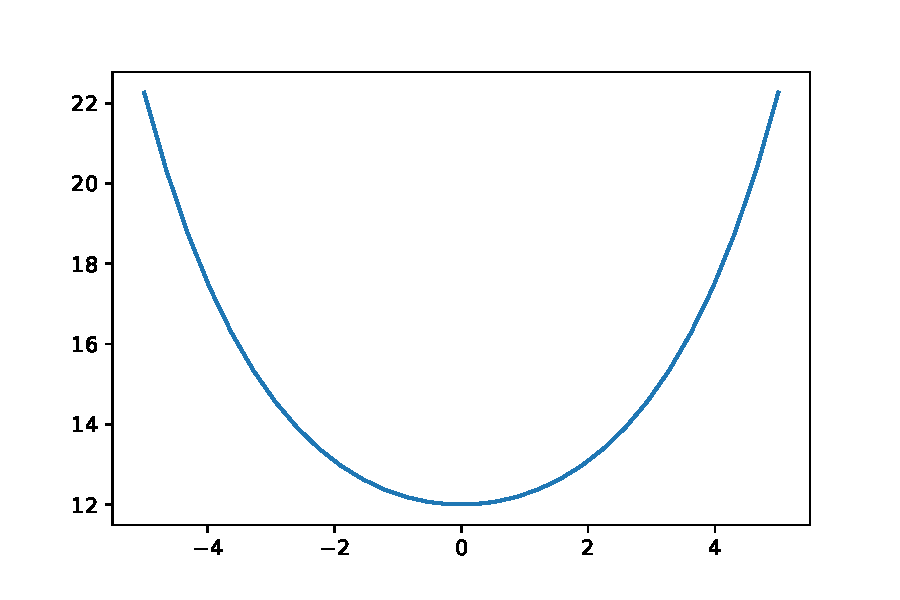
\includegraphics[scale=0.5]{code/fig3}
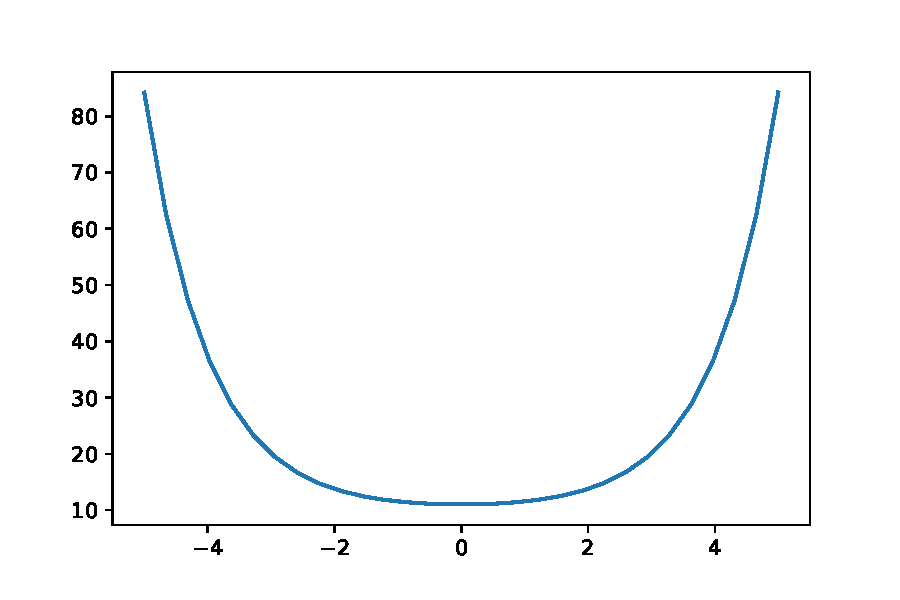
\includegraphics[scale=0.5]{code/fig4}
\caption{Det ses at en ændring fra $\lambda=2$ til $\lambda=1$ ændrer kædelinjen, både i forhold til højden af pælene og kædens hældning.}
\end{figure}
%